\subsection{FLOps Image Builder Details}

This subsection showcases how the FLOps image builder service concretely builds its different images.
The following expands upon Figure \ref{fig:flops_simple_image_builder} from \ref{subsection:flops_overview}.

\begin{figure}[p]
    \begin{adjustwidth}{-0.1\paperwidth}{-0.1\paperwidth}
        \centering
        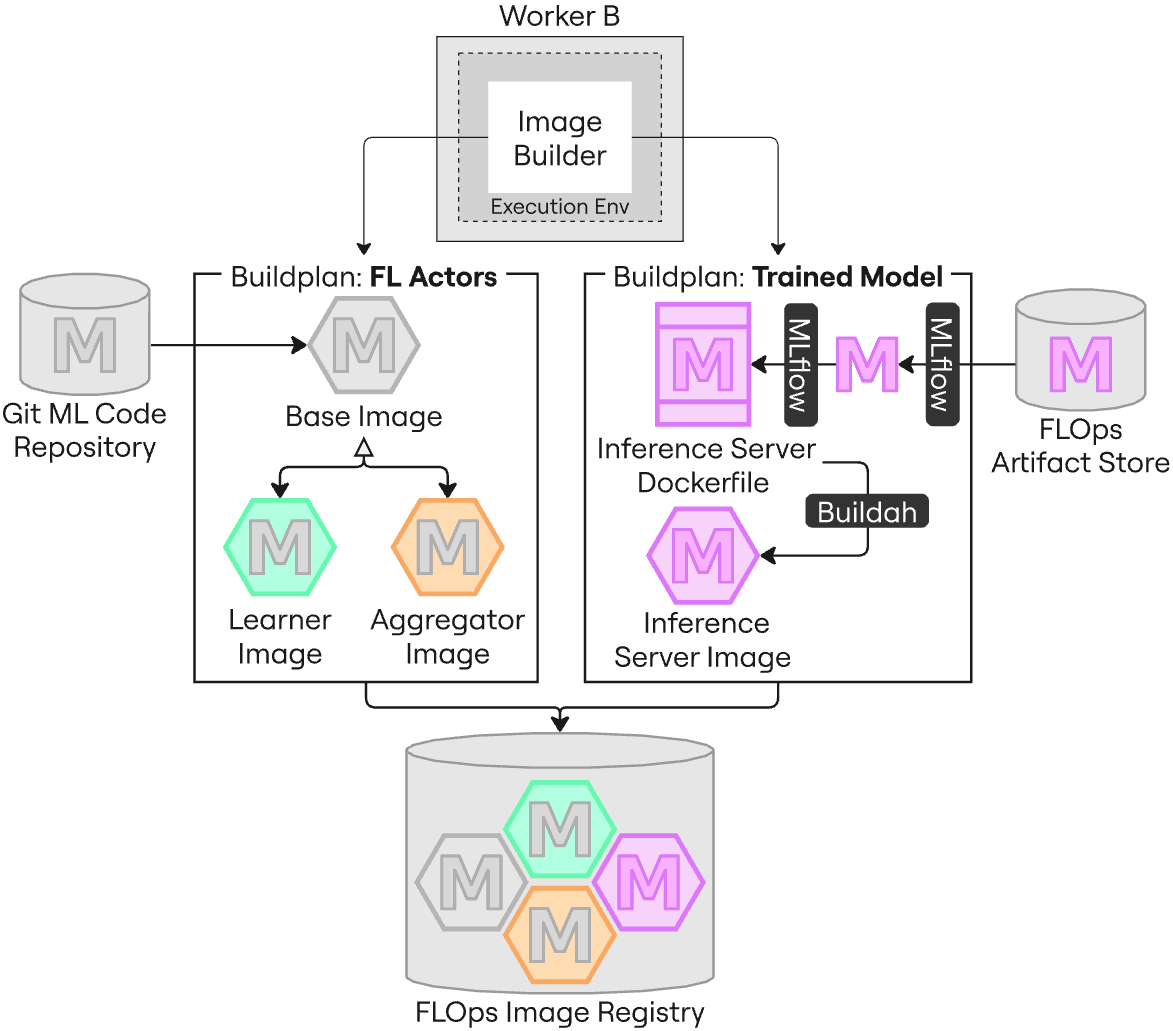
\includegraphics[width=0.80\paperwidth]{detailed_builder.png}
        \caption{Detailed FLOps Image Builder Processes}
        \label{fig:detailed_builder}
    \end{adjustwidth}
\end{figure}

Figure \ref{fig:detailed_builder} depicts the details how FLOps Image Builder works.
The grey Ms represent the untrained model (structure).
Purple Ms stand for the trained model.
Hexagons symbolize container images.
The service tracks the time different steps take and returns to the FLOps manager a summary of its total runtime and the runtime of individual steps.
The image builder supports two different build plans.

The first step in the FL Actors build plan is to fetch the user's ML code from his specified repository.
Secondly, the service builds a base image that contains all dependencies common to the learner and aggregator.
Due to the current multi-platform solution, the service pushes the base image to the image registry hosted in FLOps management.
Building and pushing the base image take up most of the service's total runtime.
The service continues to build the FL actor images one after another, pushing them in the end.
Thanks to the base image, these steps are relatively quick.
Pushing the base image does not generate meaningful overhead because of image layer caching.
The FL actor images reuse all the base image layers.
Thus, pushing them is accelerated, and the image registry recognizes and reuses its base image copy's layers.

Flower's design does not require the aggregator to possess any information about the model, including its structure or dependencies.
The aggregator's job is to average the received model parameters.
This process is based on simple mathematics and requires no other model-specific information or dependencies.
Therefore, the aggregator image and node can be relatively lightweight compared to the learners.
However, logging the trained model via MLflow requires access to the complete trained model, especially its structure.
The corresponding dependencies are necessary because a model structure is defined in a concrete ML framework.
Therefore, FLOps explicitly also includes these dependencies and the model structure in the aggregator.
During FL training only the model parameters are transmitted.
The aggregator's model copy is only needed at the very end of training.
The aggregator populates its untrained model copy via its final global model parameters.
This populated model gets logged.
Note that the model structure is initially defined in the user's ML repository and can be easily cloned and injected into images via the builder service.

The trained model build plan can only be run after the FL training is completed and the trained model is saved in the artifact store, which is hosted in the FLOps management.
MLflow provides commands to turn stored models into containers \cite{docs:mlfow_docker_cmds}.
The issue with this approach is that MLflow only provides this capability via Docker for all these commands, including building.
This approach works well directly on host machines but not inside containers (\ref{subsection:image_builders}).
As a workaround, FLOps uses MLflow to pull the stored trained model into the builder container.
Then, the service uses MLflow again to create a dockerfile based on this model.
FLOps' builder service augments this dockerfile to support multiple platforms and builds the trained model image via Buildah.
This built image wraps the trained model via an inference server.
One optional FLOps post-training step deploys this inference server directly after the builder service terminates.

\begin{figure}[b]
    \begin{changemargin}{0cm}{0cm}
        \centering
        \begin{tabular}{|c||c|c|c|c|c|c|}
            \hline
                \textbf{Image} & Image Builder & MLflow & Client & Server & SuperNode & SuperLink \\
            \hline
                \textbf{Size} & 3.0 GB & 819 MB & 1.16 GB & 1.13 GB & 232 MB & 232 MB
            \\
            \hline
        \end{tabular}
        \captionof{table}{Important FLOps Image Sizes (30.08.2024)} 
        \label{table:relevant_image_sizes_for_building}
    \end{changemargin}
\end{figure}

Table \ref{table:relevant_image_sizes_for_building} shows the sizes of different relevant images to provide more context for the final results and build processes.
The Image Builder image is the FLOps builder service.
It is noteworthy that FLOps' builder service without the MLflow (2.12.1) dependency is 900 MB and the official MLflow image is 819 MB.
The increase of more than 2.4 GB only due to this dependency is worth investigating.
The remaining images from the table are all from Flower \cite{flower_images}.
Flower recently introduced a significant change (Flower Next API \cite{docs:flower_next}) in how they use FL clients and servers.
They plan to deprecate the old approach that FLOps is using.
We tried migrating to the new Flower paradigm but encountered several issues with our current implementation.
Explaining Flower Next and FLOps' challenges with it would bloat this thesis.
This aspect is a great topic for future FLOps improvements.
The client and server images from the table are deprecated.
Their new replacements are the SuperNode and SuperLink, which are significantly smaller.
We mention these images to compare them with FLOps' FL actor images.

\begin{figure}[t]
    \begin{changemargin}{0cm}{0cm}
        \centering
        \begin{tabular}{|c|c|c|c|c|c|}
            \hline
                \textbf{Standalone} & \textbf{Base} & \textbf{Learner} & \textbf{Aggregator} & \textbf{Total Process} & \textbf{Base Image Build} \\
            \hline
                515 MB & 2.79 GB & 2.79 GB & 3.55 GB & 6min 20s & 3min 53s
            \\
            \hline
        \end{tabular}
        \captionof{table}{Simple Scikit-learn MNIST Build Example} 
        \label{table:sklearn_mnist_build_example}
    \end{changemargin}
\end{figure}
Table \ref{table:sklearn_mnist_build_example} shows a singular example of running a FLOps project using Scikit-learn and the MNIST dataset.
The Standalone refers to the standalone Scikit-learn image from Table \ref{table:ml_libs_images_compared}.
The base and learner images are equally large because the learner image only changes the files it works with but reuses all dependencies from the base image.
Therefore, the aggregator has a superset of the learner dependencies.
The total execution time for the builder service took 6 minutes and 20 seconds.
The base image build alone took almost four minutes.

FLOps Management uses and hosts an instance of the open-source CNCF (Cloud Native Computing Foundation) Distribution Registry \cite{docs:cncf_distribution_registry}.
This registry allows FLOps to be independent of any other registry provider.
FLOps has complete control and immediate access to this registry.
